% Options for packages loaded elsewhere
\PassOptionsToPackage{unicode}{hyperref}
\PassOptionsToPackage{hyphens}{url}
\PassOptionsToPackage{dvipsnames,svgnames,x11names}{xcolor}
%
\documentclass[
  letterpaper,
  DIV=11,
  numbers=noendperiod]{scrartcl}

\usepackage{amsmath,amssymb}
\usepackage{iftex}
\ifPDFTeX
  \usepackage[T1]{fontenc}
  \usepackage[utf8]{inputenc}
  \usepackage{textcomp} % provide euro and other symbols
\else % if luatex or xetex
  \usepackage{unicode-math}
  \defaultfontfeatures{Scale=MatchLowercase}
  \defaultfontfeatures[\rmfamily]{Ligatures=TeX,Scale=1}
\fi
\usepackage{lmodern}
\ifPDFTeX\else  
    % xetex/luatex font selection
\fi
% Use upquote if available, for straight quotes in verbatim environments
\IfFileExists{upquote.sty}{\usepackage{upquote}}{}
\IfFileExists{microtype.sty}{% use microtype if available
  \usepackage[]{microtype}
  \UseMicrotypeSet[protrusion]{basicmath} % disable protrusion for tt fonts
}{}
\makeatletter
\@ifundefined{KOMAClassName}{% if non-KOMA class
  \IfFileExists{parskip.sty}{%
    \usepackage{parskip}
  }{% else
    \setlength{\parindent}{0pt}
    \setlength{\parskip}{6pt plus 2pt minus 1pt}}
}{% if KOMA class
  \KOMAoptions{parskip=half}}
\makeatother
\usepackage{xcolor}
\setlength{\emergencystretch}{3em} % prevent overfull lines
\setcounter{secnumdepth}{-\maxdimen} % remove section numbering
% Make \paragraph and \subparagraph free-standing
\makeatletter
\ifx\paragraph\undefined\else
  \let\oldparagraph\paragraph
  \renewcommand{\paragraph}{
    \@ifstar
      \xxxParagraphStar
      \xxxParagraphNoStar
  }
  \newcommand{\xxxParagraphStar}[1]{\oldparagraph*{#1}\mbox{}}
  \newcommand{\xxxParagraphNoStar}[1]{\oldparagraph{#1}\mbox{}}
\fi
\ifx\subparagraph\undefined\else
  \let\oldsubparagraph\subparagraph
  \renewcommand{\subparagraph}{
    \@ifstar
      \xxxSubParagraphStar
      \xxxSubParagraphNoStar
  }
  \newcommand{\xxxSubParagraphStar}[1]{\oldsubparagraph*{#1}\mbox{}}
  \newcommand{\xxxSubParagraphNoStar}[1]{\oldsubparagraph{#1}\mbox{}}
\fi
\makeatother

\usepackage{color}
\usepackage{fancyvrb}
\newcommand{\VerbBar}{|}
\newcommand{\VERB}{\Verb[commandchars=\\\{\}]}
\DefineVerbatimEnvironment{Highlighting}{Verbatim}{commandchars=\\\{\}}
% Add ',fontsize=\small' for more characters per line
\usepackage{framed}
\definecolor{shadecolor}{RGB}{241,243,245}
\newenvironment{Shaded}{\begin{snugshade}}{\end{snugshade}}
\newcommand{\AlertTok}[1]{\textcolor[rgb]{0.68,0.00,0.00}{#1}}
\newcommand{\AnnotationTok}[1]{\textcolor[rgb]{0.37,0.37,0.37}{#1}}
\newcommand{\AttributeTok}[1]{\textcolor[rgb]{0.40,0.45,0.13}{#1}}
\newcommand{\BaseNTok}[1]{\textcolor[rgb]{0.68,0.00,0.00}{#1}}
\newcommand{\BuiltInTok}[1]{\textcolor[rgb]{0.00,0.23,0.31}{#1}}
\newcommand{\CharTok}[1]{\textcolor[rgb]{0.13,0.47,0.30}{#1}}
\newcommand{\CommentTok}[1]{\textcolor[rgb]{0.37,0.37,0.37}{#1}}
\newcommand{\CommentVarTok}[1]{\textcolor[rgb]{0.37,0.37,0.37}{\textit{#1}}}
\newcommand{\ConstantTok}[1]{\textcolor[rgb]{0.56,0.35,0.01}{#1}}
\newcommand{\ControlFlowTok}[1]{\textcolor[rgb]{0.00,0.23,0.31}{\textbf{#1}}}
\newcommand{\DataTypeTok}[1]{\textcolor[rgb]{0.68,0.00,0.00}{#1}}
\newcommand{\DecValTok}[1]{\textcolor[rgb]{0.68,0.00,0.00}{#1}}
\newcommand{\DocumentationTok}[1]{\textcolor[rgb]{0.37,0.37,0.37}{\textit{#1}}}
\newcommand{\ErrorTok}[1]{\textcolor[rgb]{0.68,0.00,0.00}{#1}}
\newcommand{\ExtensionTok}[1]{\textcolor[rgb]{0.00,0.23,0.31}{#1}}
\newcommand{\FloatTok}[1]{\textcolor[rgb]{0.68,0.00,0.00}{#1}}
\newcommand{\FunctionTok}[1]{\textcolor[rgb]{0.28,0.35,0.67}{#1}}
\newcommand{\ImportTok}[1]{\textcolor[rgb]{0.00,0.46,0.62}{#1}}
\newcommand{\InformationTok}[1]{\textcolor[rgb]{0.37,0.37,0.37}{#1}}
\newcommand{\KeywordTok}[1]{\textcolor[rgb]{0.00,0.23,0.31}{\textbf{#1}}}
\newcommand{\NormalTok}[1]{\textcolor[rgb]{0.00,0.23,0.31}{#1}}
\newcommand{\OperatorTok}[1]{\textcolor[rgb]{0.37,0.37,0.37}{#1}}
\newcommand{\OtherTok}[1]{\textcolor[rgb]{0.00,0.23,0.31}{#1}}
\newcommand{\PreprocessorTok}[1]{\textcolor[rgb]{0.68,0.00,0.00}{#1}}
\newcommand{\RegionMarkerTok}[1]{\textcolor[rgb]{0.00,0.23,0.31}{#1}}
\newcommand{\SpecialCharTok}[1]{\textcolor[rgb]{0.37,0.37,0.37}{#1}}
\newcommand{\SpecialStringTok}[1]{\textcolor[rgb]{0.13,0.47,0.30}{#1}}
\newcommand{\StringTok}[1]{\textcolor[rgb]{0.13,0.47,0.30}{#1}}
\newcommand{\VariableTok}[1]{\textcolor[rgb]{0.07,0.07,0.07}{#1}}
\newcommand{\VerbatimStringTok}[1]{\textcolor[rgb]{0.13,0.47,0.30}{#1}}
\newcommand{\WarningTok}[1]{\textcolor[rgb]{0.37,0.37,0.37}{\textit{#1}}}

\providecommand{\tightlist}{%
  \setlength{\itemsep}{0pt}\setlength{\parskip}{0pt}}\usepackage{longtable,booktabs,array}
\usepackage{calc} % for calculating minipage widths
% Correct order of tables after \paragraph or \subparagraph
\usepackage{etoolbox}
\makeatletter
\patchcmd\longtable{\par}{\if@noskipsec\mbox{}\fi\par}{}{}
\makeatother
% Allow footnotes in longtable head/foot
\IfFileExists{footnotehyper.sty}{\usepackage{footnotehyper}}{\usepackage{footnote}}
\makesavenoteenv{longtable}
\usepackage{graphicx}
\makeatletter
\def\maxwidth{\ifdim\Gin@nat@width>\linewidth\linewidth\else\Gin@nat@width\fi}
\def\maxheight{\ifdim\Gin@nat@height>\textheight\textheight\else\Gin@nat@height\fi}
\makeatother
% Scale images if necessary, so that they will not overflow the page
% margins by default, and it is still possible to overwrite the defaults
% using explicit options in \includegraphics[width, height, ...]{}
\setkeys{Gin}{width=\maxwidth,height=\maxheight,keepaspectratio}
% Set default figure placement to htbp
\makeatletter
\def\fps@figure{htbp}
\makeatother
% definitions for citeproc citations
\NewDocumentCommand\citeproctext{}{}
\NewDocumentCommand\citeproc{mm}{%
  \begingroup\def\citeproctext{#2}\cite{#1}\endgroup}
\makeatletter
 % allow citations to break across lines
 \let\@cite@ofmt\@firstofone
 % avoid brackets around text for \cite:
 \def\@biblabel#1{}
 \def\@cite#1#2{{#1\if@tempswa , #2\fi}}
\makeatother
\newlength{\cslhangindent}
\setlength{\cslhangindent}{1.5em}
\newlength{\csllabelwidth}
\setlength{\csllabelwidth}{3em}
\newenvironment{CSLReferences}[2] % #1 hanging-indent, #2 entry-spacing
 {\begin{list}{}{%
  \setlength{\itemindent}{0pt}
  \setlength{\leftmargin}{0pt}
  \setlength{\parsep}{0pt}
  % turn on hanging indent if param 1 is 1
  \ifodd #1
   \setlength{\leftmargin}{\cslhangindent}
   \setlength{\itemindent}{-1\cslhangindent}
  \fi
  % set entry spacing
  \setlength{\itemsep}{#2\baselineskip}}}
 {\end{list}}
\usepackage{calc}
\newcommand{\CSLBlock}[1]{\hfill\break\parbox[t]{\linewidth}{\strut\ignorespaces#1\strut}}
\newcommand{\CSLLeftMargin}[1]{\parbox[t]{\csllabelwidth}{\strut#1\strut}}
\newcommand{\CSLRightInline}[1]{\parbox[t]{\linewidth - \csllabelwidth}{\strut#1\strut}}
\newcommand{\CSLIndent}[1]{\hspace{\cslhangindent}#1}

\KOMAoption{captions}{tableheading}
\makeatletter
\@ifpackageloaded{caption}{}{\usepackage{caption}}
\AtBeginDocument{%
\ifdefined\contentsname
  \renewcommand*\contentsname{Table of contents}
\else
  \newcommand\contentsname{Table of contents}
\fi
\ifdefined\listfigurename
  \renewcommand*\listfigurename{List of Figures}
\else
  \newcommand\listfigurename{List of Figures}
\fi
\ifdefined\listtablename
  \renewcommand*\listtablename{List of Tables}
\else
  \newcommand\listtablename{List of Tables}
\fi
\ifdefined\figurename
  \renewcommand*\figurename{Figure}
\else
  \newcommand\figurename{Figure}
\fi
\ifdefined\tablename
  \renewcommand*\tablename{Table}
\else
  \newcommand\tablename{Table}
\fi
}
\@ifpackageloaded{float}{}{\usepackage{float}}
\floatstyle{ruled}
\@ifundefined{c@chapter}{\newfloat{codelisting}{h}{lop}}{\newfloat{codelisting}{h}{lop}[chapter]}
\floatname{codelisting}{Listing}
\newcommand*\listoflistings{\listof{codelisting}{List of Listings}}
\makeatother
\makeatletter
\makeatother
\makeatletter
\@ifpackageloaded{caption}{}{\usepackage{caption}}
\@ifpackageloaded{subcaption}{}{\usepackage{subcaption}}
\makeatother

\ifLuaTeX
  \usepackage{selnolig}  % disable illegal ligatures
\fi
\usepackage{bookmark}

\IfFileExists{xurl.sty}{\usepackage{xurl}}{} % add URL line breaks if available
\urlstyle{same} % disable monospaced font for URLs
\hypersetup{
  pdftitle={Rapport de stage 3A: Machine Learning appliqué à la cybersécurité},
  pdfauthor={Mathieu Thomassin},
  pdfkeywords={cybersécurité, machine learning, stage, rapport},
  colorlinks=true,
  linkcolor={blue},
  filecolor={Maroon},
  citecolor={Blue},
  urlcolor={Blue},
  pdfcreator={LaTeX via pandoc}}


\title{Rapport de stage 3A: Machine Learning appliqué à la
cybersécurité}
\author{Mathieu Thomassin}
\date{2024-08-31}

\begin{document}
\maketitle


\href{index.pdf}{Download PDF}

\subsection{Table des matières}\label{table-des-matiuxe8res}

\begin{itemize}
\tightlist
\item
  \hyperref[introduction]{Introduction}
\item
  \hyperref[duxe9couverte-et-contexte]{01 - Découverte et Contexte}
\item
  \hyperref[recherche-et-collecte-de-donnuxe9es]{02 - Recherche et
  Collecte de Données}
\item
  \hyperref[choix-des-probluxe8mes-et-des-outils-de-machine-learning]{03
  - Choix des Problèmes et des Outils de Machine Learning}
\item
  \hyperref[exploration-de-moduxe8les-et-outils-avancuxe9s]{04 -
  Exploration de Modèles et Outils Avancés}
\item
  \hyperref[anomaly-detection-et-moduxe8les-de-classification]{05 -
  Anomaly Detection et Modèles de Classification}
\item
  \hyperref[exploration-darticles-scientifiques]{06 - Exploration
  d'Articles Scientifiques}
\item
  \hyperref[moduxe9lisation-et-uxe9valuation-des-moduxe8les]{07 -
  Modélisation et Évaluation des Modèles}
\item
  \hyperref[travail-avec-splunk-et-pipelines]{08 - Travail avec Splunk
  et Pipelines}
\item
  \hyperref[expuxe9rimentations-et-duxe9ploiement]{09 - Expérimentations
  et Déploiement}
\item
  \hyperref[reproductibilituxe9-et-mlops]{10 - Reproductibilité et
  MLOps}
\item
  \hyperref[conclusion]{Conclusion}
\item
  \hyperref[annexe]{Annexe}
\end{itemize}

\subsection{Présentation du stagiaire et du maître de
stage}\label{pruxe9sentation-du-stagiaire-et-du-mauxeetre-de-stage}

\begin{itemize}
\tightlist
\item
  \textbf{Stagiaire} : Mathieu THOMASSIN
\item
  \textbf{Maître de stage} : Michael ORSUCCI, responsable du
  \emph{Security Operation Center} de l'Insee
\item
  \textbf{Titre du stage} : Machine Learning appliqué à la cybersécurité
\end{itemize}

\subsection{Introduction}\label{introduction}

L'Insee a renforcé récemment ses capacités opérationnelles en termes de
cybersécurité via notamment la création de son SOC (Security Operation
Center) en septembre 2023. Devant la quantité de données et leur
diversité et face aux évolutions des techniques et tactiques des
attaquants, les méthodes de détection de cyberattaques peuvent avoir des
limites. L'application d'algorithmes de Machine Learning peut aider les
analystes SOC à repérer des attaques. Se déroulant au sein de l'équipe
SOC construite depuis peu, le stage va permettre d'appliquer des
techniques de Machine Learning et de deep learning sur des jeux de
données réelles, afin de participer à la détection d'incidents de
sécurité.

\subsubsection{Présentation de
l'organisation}\label{pruxe9sentation-de-lorganisation}

L'Insee a renforcé récemment ses capacités opérationnelles en termes de
cybersécurité via notamment la création de son SOC (Security Operation
Center) en septembre 2023. Cette équipe est répartie entre les sites de
la DR de Nantes et la DR de Metz et a pour objectif de renforcer la
sécurité du système d'information (SI).

\subsubsection{Contexte général du
stage}\label{contexte-guxe9nuxe9ral-du-stage}

Devant la quantité de données et leur diversité et face aux évolutions
des techniques et tactiques des attaquants, les méthodes de détection de
cyberattaques peuvent avoir des limites. L'application d'algorithmes de
Machine Learning peut aider les analystes SOC à repérer des attaques. Le
stage avait donc pour but de permettre d'appliquer des techniques de
Machine Learning et de deep learning sur des jeux de données réelles,
afin de participer à la détection d'incidents de sécurité.

\subsubsection{Objectifs du stage}\label{objectifs-du-stage}

\paragraph{Objectifs principaux}\label{objectifs-principaux}

Il s'agissait d'appliquer des techniques de détection de requêtes
malveillantes arrivant dans le SI de l'Insee. Les requêtes arrivant au
sein du SI peuvent être centralisées par un SIEM (Security Information
and Event Management).

\paragraph{Résultats attendus}\label{ruxe9sultats-attendus}

\begin{itemize}
\tightlist
\item
  Offrir un service s'ajoutant au SIEM permettant d'identifier des
  requêtes malveillantes.
\item
  Pouvoir comparer différents meilleurs modèles (au sens d'une recherche
  dans les hyperparamètres) entre eux.
\item
  Favoriser les bonnes pratiques du MLOps : reproductibilité, contrôle
  de version, automatisation, surveillance, collaboration.
\item
  Étendre la méthodologie à des jeux de données publics différents.
\item
  Explorer les algorithmes de détection d'anomalie.
\end{itemize}

\subsubsection{Importance de la mission pour
l'Insee}\label{importance-de-la-mission-pour-linsee}

À titre d'exemple, l'Insee détient l'application Elire. Une attaque
réussie sur cette application perturberait le bon déroulement de la vie
démocratique. Finaliser la formation d'attaché statisticien en
s'appliquant à résoudre un problème concret avant une prise de poste
dans un domaine proche.

\subsubsection{Contexte général du
stage}\label{contexte-guxe9nuxe9ral-du-stage-1}

Ce stage s'inscrit pleinement dans le parcours que j'ai progressivement
construit tout au long de ma carrière à l'Insee. Débutant il y a
plusieurs années sur un poste de contrôleur-programmeur, j'ai pu
apprécier les cours d'informatique et de statistiques pendant mon
parcours à l'Ensai. J'y ai suivi les options menant progressivement à se
spécialiser jusqu'au master en Informatique et traitement des données.

Au cours de ma préparation et de l'obtention de la qualification
d'analyste, ma curiosité pour la sécurité des systèmes d'information
s'est particulièrement développée. L'analyse des requêtes au sein d'un
réseau soulève de nombreuses questions : volume des données, méthode de
traitement statistique avec le machine learning, rapidité et efficacité
de ce traitement. C'est un domaine où les techniques de machine learning
présentent un intérêt certain.

Les enjeux de la cybersécurité peuvent se révéler particulièrement
lourds, comme on peut le découvrir dans les journaux pour de nombreuses
organisations. Ce stage au SOC représente une opportunité unique de
confronter ces intérêts théoriques à des problématiques concrètes de
cybersécurité, renforçant ainsi mes compétences et ma compréhension dans
un domaine en pleine expansion.

\subsubsection{Importance de la cybersécurité et du machine learning
dans ce
domaine}\label{importance-de-la-cybersuxe9curituxe9-et-du-machine-learning-dans-ce-domaine}

La cybersécurité et le machine learning sont cruciaux pour les
entreprises aujourd'hui pour plusieurs raisons. D'une part, la
cybersécurité est essentielle pour protéger les données sensibles contre
les cyberattaques qui sont de plus en plus sophistiquées et fréquentes.
Les conséquences d'une faille de sécurité peuvent être dévastatrices
pour l'Insee, incluant des pertes de données, des dommages à la
réputation et la crédibilité de l'Institut, et des impacts sur les
utilisateurs.

D'autre part, le machine learning offre des outils puissants pour
détecter et prévenir les menaces en temps réel. Grâce à ses capacités de
traitement et d'analyse de vastes quantités de données, le machine
learning peut identifier des modèles et des anomalies que les méthodes
traditionnelles pourraient manquer. Par exemple, la DSI a déployé sur le
poste de chaque agent HarfangLab, un outil de sécurité informatique
reposant sur des modèles de machine learning pour détecter la présence
de logiciels malveillants, des malware, et permettant d'isoler le poste
compromis.

\begin{figure}[H]

{\centering 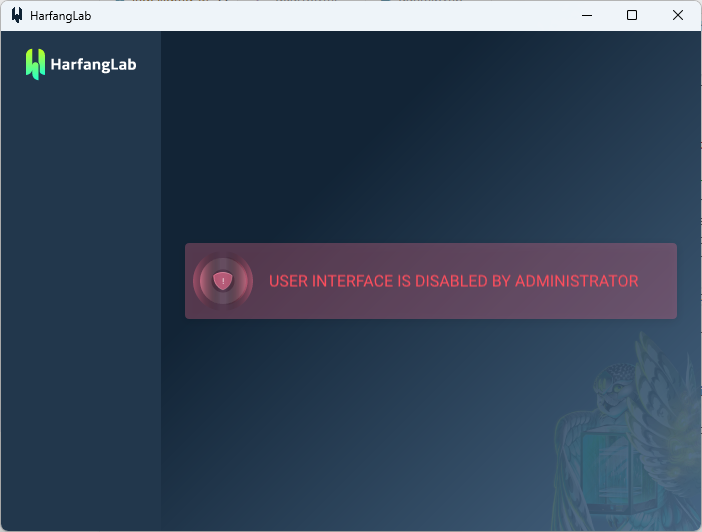
\includegraphics[width=0.4\textwidth,height=\textheight]{figures/HarfangLab.png}

}

\caption{HarfangLab, déployé sur le poste de travail}

\end{figure}%

Le machine learning permettrait également de réduire le travail des
analystes du SOC en classifiant automatiquement les requêtes comme
bégnines ou malveillante.

\subsubsection{Objectifs du stage}\label{objectifs-du-stage-1}

En débutant ce stage, j'avais pour but de pouvoir réaliser des objectifs
à la fois académiques, en lien avec mes intérêts développés lors de la
scolarité, ainsi que des objectifs professionnels, me permettant de
m'insérer au mieux dans la structure de l'Insee pour débuter ma carrière
d'attaché.

\begin{enumerate}
\def\labelenumi{\arabic{enumi}.}
\item
  \textbf{Alignement avec mes objectifs de carrière} : Ce stage
  présentait une opportunité unique de développer des compétences à la
  fois en statistique et en informatique. De plus, au lieu de se
  dérouler dans un service de développement, il a eu lieu dans un
  service de production, ce qui m'a permis de découvrir une autre
  perspective de l'informatique par rapport à l'informatique de type
  ``data science'' pratiquée à l'Ensai. En renforçant mes compétences en
  machine learning et en informatique, j'ai donc pu acquérir de
  l'expérience pour de futurs rôles au sein de l'Insee.
\item
  \textbf{Développement de compétences spécifiques} : Pour réaliser la
  tâche principale de ce stage, j'avais besoin de maîtriser des
  techniques de machine learning et de deep learning appliquées à la
  cybersécurité, ainsi que de les inscrire dans une approche de type
  DevOps ou MLOps. Il m'a donc fallu utiliser des outils comme
  Scikit-learn, MLflow, des techniques de deep learning, et utiliser le
  cluster Kubernetes pour entraîner et déployer un modèle avec une API.
\item
  \textbf{Application pratique des connaissances théoriques} : Si j'ai
  appris à faire du machine learning à l'école et y ai découvert des
  notions de DevOps, ce n'est qu'en arrivant en stage que j'ai pu
  découvrir l'étendue des problèmes pratiques que cela peut poser.
  Isolés, dans des environnements de travail bien conçus, voire
  seulement à travers une présentation théorique, les cours m'ont permis
  d'acquérir des connaissances. Cependant, c'est seulement en
  travaillant sur des projets réels que j'ai pu répondre de façon
  pratique en piochant dans la boîte à outils de mes cours.
\item
  \textbf{Contribution à l'organisation d'accueil} : Débutant dans le
  domaine de la cybersécurité, je n'avais pas pour objectif d'apporter
  une solution exploitable en production. En revanche, il était
  essentiel pour moi de démontrer ma capacité future à prendre une
  position d'ingénieur capable d'envisager un problème nouveau et d'y
  apporter une solution pratique exploitable par une équipe. La création
  d'un socle d'entraînement pour un modèle de détection de requêtes
  malveillantes, destiné à être utilisé par des utilisateurs, sert cet
  objectif.
\item
  \textbf{Exploration des défis et opportunités} : Face à un nouveau
  problème pour moi, j'ai voulu prendre le temps d'explorer certaines
  spécificités liées à la cybersécurité et les pratiques MLOps. J'ai
  donc recherché, à travers le web, dans des livres et des articles, les
  méthodes classiques en machine learning pour améliorer la sécurité des
  systèmes d'information ainsi que les façons possibles de les mettre en
  œuvre de manière robuste et reproductible.
\end{enumerate}

Ces objectifs m'ont permis de m'assurer que ce stage serait bénéfique
pour mon parcours comme pour l'Insee. Cependant, s'ils apparaissent
rétrospectivement relativement clairs, ils ont pourtant été construits
au fur et à mesure de mon avancée comme nous allons maintenant
l'explorer.

\subsection{1. Découverte et Contexte}\label{duxe9couverte-et-contexte}

\subsubsection{Premiers pas dans le stage : Enthousiasme et
incertitude}\label{premiers-pas-dans-le-stage-enthousiasme-et-incertitude}

\begin{itemize}
\item
  \textbf{Sentiments initiaux} : Avant de commencer le stage, j'avais pu
  discuter avec le RSSI (Responsable Sécurité du Système d'Information)
  et le DSI (Directeur du Système d'Information) de l'Insee au cours
  d'une formation interne avant l'oral de la qualification d'analyste.
  J'étais plutôt impressionné par les enjeux, le SI de l'Insee étant
  régulièrement la cible d'attaques dont j'entendais parler. Cependant,
  si je savais que je n'étais pas formé comme un ``véritable''
  informaticien (n.d.), n'ayant reçu qu'une ``sensibilisation à
  l'informatique de production ou à la sécurité'' (n.d.) p55, j'avais
  plutôt confiance dans mes récentes capacités à traiter des données et
  dans mon envie de découvrir le domaine.
\item
  \textbf{Raisons de ces sentiments} : Lors de la scolarité, j'avais
  pris l'habitude d'explorer les rayonnages de la bibliothèque de
  l'Ensai, et j'y avais repéré un livre (n.d.) sur le machine learning
  et la sécurité. Me remémorant ce dont m'avait parlé mon ancien maître
  de stage sur le plan de reprise d'activité de l'application critique
  Elire, et en sachant qu'un système informatique génère une quantité de
  données sur lesquelles il est possible de travailler pour mieux en
  comprendre les rouages, la perspective de travailler sur la sécurité
  du SI de l'Insee m'intéressait beaucoup. Cependant, je n'avais pas
  encore d'idée sur l'application concrète d'un tel projet, ce qui me
  plongeait dans une certaine incertitude.
\item
  \textbf{Objectifs personnels initiaux} : C'est pourquoi, j'avais tout
  d'abord comme objectif de mieux comprendre ce qu'il était possible de
  faire en sécurité informatique au sein de l'Insee. N'y avait-il pas
  déjà des outils externes très performants ? Qu'était-il possible
  d'apporter en tant qu'attaché statisticien débutant ?
\end{itemize}

\subsubsection{Introduction à la cybersécurité : Définition et
importance}\label{introduction-uxe0-la-cybersuxe9curituxe9-duxe9finition-et-importance}

\begin{itemize}
\item
  \textbf{Définition de la cybersécurité} : La cybersécurité consiste à
  protéger les systèmes, les réseaux et les programmes contre les
  attaques numériques. (n.d.) Elle vise à garantir la confidentialité,
  l'intégrité et la disponibilité des informations. Assurer la sécurité
  du système d'information (SSI) consiste à gérer les risques de
  sécurité selon une démarche en trois étapes: lister, évaluer et
  traiter les risques. (n.d.) La notion de SOC, \emph{Security Operation
  Center}, devient alors essentiel pour mettre en oeuvre une politique
  de cybersécurité. UN SOC, doit ``monitorer l'ensemble des composants
  d'un système d'information et être capable de détecter et de
  sélectionner parmi des milliards d'octets des éléments caractéritiques
  d'une cyberattaque'' (2024).
\item
  \textbf{Importance de la cybersécurité} : Une attaque informatique a
  aujourd'hui d'autant plus de valeur que l'activité des organisations
  est pratiquement toujours menée à l'aide d'outils informatiques. Sans
  défendre correctement cet outil, la continuité de l'activité est
  menacée d'interruption plus ou moins forte. La cybersécurité cherche
  également à protéger les données sensibles et personnelles, notamment
  au travers de l'obligation légale issue du Règlement Général sur la
  Protection des Données (RGPD). La confiance que le grand public
  accorde à l'Insee serait amoindrie en cas d'attaque réussie. C'est
  pourquoi la cybersécurité doit faire l'objet d'un soin permanent par
  l'Insee.
\item
  \textbf{Liens avec le machine learning} : La cybersécurité est très
  naturellement un domaine d'application du machine learning. En effet,
  on peut y obtenir des jeux de données robustes qui permettront
  ``d'annuler certains des progrès les plus complexes dans la compétence
  des attaquants''. Le machine learning peut ainsi améliorer ou
  remplacer les ``solutions basées sur des règles dans des problèmes
  comme la détection d'intrusion, la classification des logiciels
  malveillants ou l'analyse réseau'' ((n.d., 5--6) ).
\end{itemize}

\subsubsection{Présentation de l'équipe SOC et du système d'information
(SI)}\label{pruxe9sentation-de-luxe9quipe-soc-et-du-systuxe8me-dinformation-si}

\paragraph{Structure de l'équipe SOC}\label{structure-de-luxe9quipe-soc}

L'équipe SOC de l'Insee a été créée en 2023 et est constituée de 6
membres répartis sur deux sites : Nantes et Metz. Son objectif principal
est d'établir et de mettre en œuvre la politique de sécurité du système
d'information (SI) de l'Insee. L'équipe est dirigée par un responsable
unique qui pilote les travaux de manière transversale entre les deux
sites. Les membres de l'équipe incluent des analystes de sécurité, des
ingénieurs en cybersécurité, et des experts en gestion des incidents.

\paragraph{Fonctionnement du SOC}\label{fonctionnement-du-soc}

L'équipe SOC a pour mission de surveiller en permanence le SI de l'Insee
afin de détecter, qualifier et remédier aux incidents de sécurité. Les
principales activités du SOC incluent (n.d.):

\begin{itemize}
\item
  \textbf{Veille et qualification des vulnérabilités} : Identifier
  quotidiennement les vulnérabilités affectant le SI de l'Insee et
  évaluer leur impact potentiel.
\item
  \textbf{Conception de solutions de sécurité} : Développer et mettre en
  place des solutions technologiques pour renforcer la sécurité du SI,
  notamment par la mise en place de solutions techniques innovantes pour
  garantir la sécurité du SI.
\item
  \textbf{Détection et gestion des incidents} : Utiliser des outils
  avancés comme le SIEM (Security Information and Event Management) ou
  des EDR (Endpoint Detection and Response) pour détecter les activités
  suspectes et les incidents de sécurité, puis élaborer et mettre en
  œuvre des plans de remédiation en collaboration avec les équipes
  concernées.
\item
  \textbf{Maintien en condition de sécurité} : Assurer la sécurité
  continue des différents systèmes d'information en surveillant les
  infrastructures et en veillant à l'application des correctifs
  nécessaires.
\item
  \textbf{Support et expertise} : Apporter une expertise en sécurité aux
  différentes unités de l'Insee, conseiller sur les meilleures pratiques
  et aider à la décision en matière de sécurité informatique.
\end{itemize}

L'équipe SOC joue un rôle crucial dans la préservation de l'intégrité,
de la confidentialité et de la disponibilité des données et des systèmes
de l'Insee. Leur travail permet de protéger les actifs numériques de
l'organisation contre une variété de menaces cybernétiques.

\begin{itemize}
\tightlist
\item
  \textbf{Présentation du SI} : Le système d'information de l'Insee est
  documenté sur un wiki interne (2024). On peut notamment y trouver des
  schémas sur l'architecture du SI de production, mais pas sur celle du
  SI d'administration. L'architecture du SIA est très fortement guidée
  par les recommandations de l'anssi. (n.d.) Pour l'essentiel, on peut
  retenir une organisation en 3 couches.
\end{itemize}

\begin{figure}[H]

{\centering 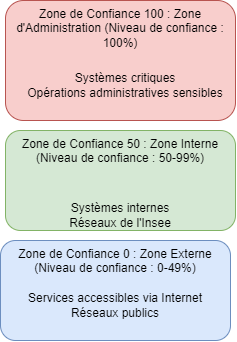
\includegraphics{figures/schema_SI_simplifie.png}

}

\caption{Schéma simplifié du Système d'Information de l'Insee}

\end{figure}%

Le plus important pour le stage étant que le SI a un unique point
d'entrée/sortie en zone 0: un firewall F5 qui permet de sécuriser et
gérer le trafic réseau. C'est une solution sophistiquée (prix de vente
global supérieur à 60 000 €) qui va protéger les applications et le
réseau contre un large éventail de menaces tout en optimisant les
performances et la disponibilité des services.

\subsubsection{Compréhension du SIEM et des
logs}\label{compruxe9hension-du-siem-et-des-logs}

\begin{itemize}
\item
  \textbf{Rôle du SIEM} : Un SIEM (Security Information and Event
  Management) est essentiel dans la conduite d'une politique de sécurité
  informatique. C'est un outil qui rassemble des données provenant de
  différentes machines du système d'information, les centralise et
  effectue des analyses sur elles. Chaque appareil du réseau génère des
  logs que l'on peut regrouper en deux types :
\item
  \textbf{Logs centrés sur l'hôte} : Capturent les événements survenus à
  l'intérieur de la machine hôte, tels qu'un utilisateur accédant à un
  fichier ou l'exécution d'un processus.
\item
  \textbf{Logs centrés sur le réseau} : Génèrent des logs lorsque les
  machines communiquent entre elles ou avec l'extérieur, comme le trafic
  web sur le site www.insee.fr, un fichier récupéré via le protocole
  FTP, ou encore un utilisateur se connectant au moyen d'un VPN.
\end{itemize}

L'importance du SIEM provient du fait que le flux des logs est très
important, de l'ordre de plusieurs dizaines de Go par jour pour le SI de
l'Insee. En cas d'incident, examiner les logs machine par machine est
une tâche pratiquement impossible sans SIEM. Il est possible de
paramétrer certaines règles qui vont permettre de créer des alarmes. Un
SIEM permet de faire des recherches dans les logs, de corréler les
événements et de répondre rapidement aux incidents grâce à un système de
détection et d'alerte en temps réel.

\begin{itemize}
\tightlist
\item
  \textbf{Utilisation des logs} : Tous les appareils du SI génèrent des
  logs comme on l'a vu. Par exemple Windows enregistre tous les
  événements, visibles sur l'Event Viewer. Chaque type de log reçoit un
  ID ce qui permet une analyse plus facile. Ces logs peuvent être
  envoyées (``forwardées'') au SIEM. On peut aussi récupérer des logs
  sur une machine Linux (ce qui concerne notamment les serveurs dans le
  SI de l'Insee). De même, il est très important de surveiller les
  requêtes et les réponses sur les serveurs webs afin de détecter des
  attaques webs. C'est un point central dans ce stage. Voici un exemple
  de ce dernier type de log
\end{itemize}

\textbf{Exemple de log issue d'une requête web :}

\begin{Shaded}
\begin{Highlighting}[]
\NormalTok{127.0.0.1 {-} {-} [21/March/2022:10:22:04 {-}0300] "GET / HTTP/1.0" 200 2216}
\end{Highlighting}
\end{Shaded}

\begin{itemize}
\tightlist
\item
  \textbf{Client IP} : 127.0.0.1 (localhost)
\item
  \textbf{Identd} : - (non utilisé)
\item
  \textbf{Utilisateur Authentifié} : - (non utilisé)
\item
  \textbf{Date et Heure} : 21 mars 2022, 10:22:04 (UTC-3)
\item
  \textbf{Demande HTTP} : GET / (utilisant HTTP/1.0)
\item
  \textbf{Code de Statut} : 200 (OK)
\item
  \textbf{Taille de la Réponse} : 2216 octets
\end{itemize}

Lorsqu'une menace atteignant le SI est détectée par le SIEM, une alerte
est lancée. Cette dernière permet aux analystes du SOC de la traiter. Un
SIEM permet donc d'obtenir une visibilité sur l'ensemble des points du
SI qui y auront été connectés. Dans le cadre du stage, j'ai pu accéder à
un test de Splunk sur la partie du SI en zone sécurisée. Ainsi, j'ai été
capable de récupérer les logs provenant du F5 positionné à l'entrée de
cette zone 50.

\subsection{2. Recherche et Collecte de
Données}\label{recherche-et-collecte-de-donnuxe9es}

\subsubsection{Attente de Splunk et recherche de datasets
pertinents}\label{attente-de-splunk-et-recherche-de-datasets-pertinents}

Au début du stage, le SIEM Splunk n'était pas encore prêt. Je ne
connaissais pas encore les données possibles. J'ai donc cherché des
exemples de machine learning dans le domaine de la cybersécurité. -
Types de données : Réseau, logs, HTTP il a fallu comprendre le type de
données sur lesquelles travailler. De nombreuses travaux sont
disponibles en cybersécurité. Il existe également un certain nombre de
datasets disponibles. Par exemple, on peut trouver des données sur des
paquets de type ``PCAP'', des jeux de données avec des tentatives
d'intrusion, des malwares ou bien des urls de sites webs malicieux. Sans
problème à résoudre bien identifié, il est compliqué de s'orienter
dedans. Voici quelques exemples de jeux de données disponibles: 1.
Frameworks and Models 2. Encrypted Traffic Analysis 3. Intrusion
Detection 4. Botnet and Ransomware 5. URL-based Threats 6. Cloud
Infrastructure Security 7. Malware Analysis 8. Network and Host Events
9. Miscellaneous Datasets

Un type de données

\subsubsection{Présentation des premières données
sélectionnées}\label{pruxe9sentation-des-premiuxe8res-donnuxe9es-suxe9lectionnuxe9es}

Le jeu de données ``good\_bad\_queries'' disponible ICI a constitué une
étape importante. En effet, ce jeu de données est très simple. Il est
constitué de deux fichiers. L'un ``good\_queries.txt'' contient des url
de requêtes http non malicieuses, et l'autre ``bad\_queries.txt''
contient des requêtes malicieuses. Ce sont des fichiers de texte, sur
une seule colonne. Voici un exemple:

La simplicité de ce jeu de données est à relativiser. Dans le cadre du
stage, il est intéressant d'apprendre à le connaître par une première
analyse descriptive. En effet, dans les données issues du firewall f5,
auxquelles j'ai eu accès plus tard, on s'aperçoit vite qu'une attaque
est avant tout portée par le contenu de ce champ. D'autres champs d'une
requête peuvent aider à déterminer s'il s'agit d'une attaque ou non,
mais sans l'url, il est pratiquement imposssible de conclure. Voici une
petite analyse descriptive de ce jeu de données:

\subsection{3. Choix des Problèmes et des Outils de Machine
Learning}\label{choix-des-probluxe8mes-et-des-outils-de-machine-learning}

recherche de sites, un bien:
https://github.com/jivoi/awesome-ml-for-cybersecurity

\subsubsection{Définition des problèmes de machine learning en
cybersécurité}\label{duxe9finition-des-probluxe8mes-de-machine-learning-en-cybersuxe9curituxe9}

faut-il faire de la détection d'anomalie (non supervisé) ou bien de la
classification (supervisée)

\subsubsection{Introduction à Scikit-learn et choix des
modèles}\label{introduction-uxe0-scikit-learn-et-choix-des-moduxe8les}

road map de scikit learn:
https://scikit-learn.org/1.3/tutorial/machine\_learning\_map/index.html

\subsubsection{Formation à l'interprétabilité des
modèles}\label{formation-uxe0-linterpruxe9tabilituxe9-des-moduxe8les}

shap: https://train.learn.datascientest.com/notebooks/137/447

\subsection{4. Exploration de Modèles et Outils
Avancés}\label{exploration-de-moduxe8les-et-outils-avancuxe9s}

\subsubsection{Essais avec XGBoost pour la classification des
malwares}\label{essais-avec-xgboost-pour-la-classification-des-malwares}

essai simple et rapide, mais hors sujet. Retour sur good bad queries

\subsubsection{Découverte de MLflow et utilisation de
l'API}\label{duxe9couverte-de-mlflow-et-utilisation-de-lapi}

Comment gérer tous ces notebook ? cf.~cours de Lino

\subsubsection{Introduction au deep learning avec le livre ``Deep
Learning from Scratch''
(DLFS)}\label{introduction-au-deep-learning-avec-le-livre-deep-learning-from-scratch-dlfs}

Bon, il va falloir faire du deep learning, mais comment s'y prendre
vraiment ? Est-ce uqe j'ai bien compris en cours ? Voyons voir. Ah oui,
on peut battre une régression linéaire avec du deep learning fait soi
même. Voir le livre.

\subsubsection{Exploration des design patterns en deep
learning}\label{exploration-des-design-patterns-en-deep-learning}

Aller voir les différences possibles dans les modèles pour implémenter
ensuite.

\subsection{5. Anomaly Detection et Modèles de
Classification}\label{anomaly-detection-et-moduxe8les-de-classification}

\subsubsection{Détour par la détection d'anomalies : Difficultés et
recentrage}\label{duxe9tour-par-la-duxe9tection-danomalies-difficultuxe9s-et-recentrage}

on peut facilement faire de la détection d'anomalie avec des algo,
l'article fondateur est disponible. Mais le sujet apparaît encore trop
difficile. Je n'ai pas encore les données, mais je peux accéder à des
dataset de requête http labellisé. Donc on va se recentrer dessus.

\subsubsection{Analyses simples avec KNN et
clustering}\label{analyses-simples-avec-knn-et-clustering}

très difficile de faire ce genre de chose, car la tokenization implique
de passer en grande (grande\ldots) dimension. Curse of dimensionality.
Le clustering ne nous intéresse pas pour répondre à un problème
d'analyste SOC. Je veux pouvoir analyser une requête, pas connaître des
clusters.

\subsubsection{Analyse des données HTTP et détection des attaques (ex.
DDOS)}\label{analyse-des-donnuxe9es-http-et-duxe9tection-des-attaques-ex.-ddos}

On ne peut pas détecter du DDOS, et ce n'est pas l'objet. Il sera trop
tard. Donc on va encore limiter à des requêtes pour d'autres attaques.

\subsubsection{Focalisation sur l'analyse des URL et compréhension des
attaques}\label{focalisation-sur-lanalyse-des-url-et-compruxe9hension-des-attaques}

quelques documents disponibles, les champs (description dans un des
articles) COmment tokenizer la données ?

\subsection{6. Exploration d'Articles
Scientifiques}\label{exploration-darticles-scientifiques}

\subsubsection{Lecture et analyse de l'article ``Machine Learning for
Cybersecurity Applications'' de la West Virginia University
(WVU)}\label{lecture-et-analyse-de-larticle-machine-learning-for-cybersecurity-applications-de-la-west-virginia-university-wvu}

\subsubsection{Étude de ``A Comprehensive Review of Anomaly Detection in
Web Logs'' du Hasso Plattner Institute
(HPI)}\label{uxe9tude-de-a-comprehensive-review-of-anomaly-detection-in-web-logs-du-hasso-plattner-institute-hpi}

Beaucoup de choses peuvent être faite dans la détection, mais finalement
pas tant de problèmes similaires au mien.

\subsubsection{Exploration de ``Conf\_SIN2022\_\_SWAF'' pour le
développement d'un pare-feu applicatif basé sur du machine
learning}\label{exploration-de-conf_sin2022__swaf-pour-le-duxe9veloppement-dun-pare-feu-applicatif-basuxe9-sur-du-machine-learning}

VOILà! ils utilisent un dataset que j'ai, avec une technique que je
comprends. On peut reproduire le réseau de neurones. Mais pas les
résultats. Cependant, leur technique de (non) tokenization est simple et
apporte un excellent résultat sur le dataset good/bad queries.

\subsection{7. Modélisation et Évaluation des
Modèles}\label{moduxe9lisation-et-uxe9valuation-des-moduxe8les}

\subsubsection{Modélisation des URL : KNN, SVM, regression logistique,
CNN}\label{moduxe9lisation-des-url-knn-svm-regression-logistique-cnn}

Certains choix s'imposent par leur simplicité ou leur rapidité.
Cependant, il faut rapidement se rendre compte que les scores f1 sont
mauvais et qu'une autre solution peut être tentée.

\subsubsection{Utilisation de ChatGPT et des GPU pour accélérer le
développement}\label{utilisation-de-chatgpt-et-des-gpu-pour-accuxe9luxe9rer-le-duxe9veloppement}

Clairement, accéder à un GPU est crucial pour l'entraînement des réseaux
de neurones. On passe parfois de 2h à 20 minutes. De son côté, CHatgpt
4o permet, par itération, de debugguer rapidement, de documenter à
grande vitesse et surtout de coder des éléments selon des spécifications
qui changent rapidement.

\subsubsection{Organisation des priorités et gestion des
expérimentations}\label{organisation-des-priorituxe9s-et-gestion-des-expuxe9rimentations}

Il a fallu commencer à développer un pipeline permettant d'utiliser
MLflow, puis de requêter le modèle taggué comme ``en production'' dans
MLflow. Cela constituait une application ``minimum''.

\subsection{8. Travail avec Splunk et
Pipelines}\label{travail-avec-splunk-et-pipelines}

\subsubsection{Traitement des données Splunk en
préproduction}\label{traitement-des-donnuxe9es-splunk-en-pruxe9production}

Splunk étant mis en test, j'ai pu manipuler le siem et me rendre compte
des données que je récupérais.

\subsubsection{Tokenization des URL et
limitations}\label{tokenization-des-url-et-limitations}

Une tokenization classique: sujette à l'imagination et source de
versions infinies. Mais dont les limites surviennent lors de la
conception du modèle. donner exemple de codes Jusqu'à l'idée de
l'article: pas de tokenization mais un passage par le code Ascii. donner
la fonction.

\subsubsection{Développement de pipelines et utilisation de
GridsearchCV}\label{duxe9veloppement-de-pipelines-et-utilisation-de-gridsearchcv}

Pour pouvoir calibrer le modèle, il faut pouvoir jouer sur les hyper
paramètres. Il a donc fallu trouver comment utiliser GridsearchCV
=\textgreater{} consommateur de temps.

\subsubsection{Évaluation des performances des
modèles}\label{uxe9valuation-des-performances-des-moduxe8les}

On peut avoir un score accuracy très élevé, mais un f1 très bas car les
classes sont déséquilibrées. pas de problème de datadrift, car pas
encore de données. Les datasets sont fixes. Mais c'est un problème.

\subsection{9. Expérimentations et
Déploiement}\label{expuxe9rimentations-et-duxe9ploiement}

\subsubsection{Utilisation de MLFlow pour la gestion des
expérimentations}\label{utilisation-de-mlflow-pour-la-gestion-des-expuxe9rimentations}

MLflow vs.~Metaflow.

\subsubsection{Apprentissage à requêter et déployer un modèle via une
API}\label{apprentissage-uxe0-requuxeater-et-duxe9ployer-un-moduxe8le-via-une-api}

utilisation de FastAPI

\subsubsection{Déploiement sur un cluster Kubernetes et gestion du
preprocessing}\label{duxe9ploiement-sur-un-cluster-kubernetes-et-gestion-du-preprocessing}

Assure une stabilité du site. Il faut reproduire le preprocessing
utilisé dans la construction du modèle pour pouvoir utiliser l'API.
construction du modèle =\textgreater{} stockage du modèle dans MLFlow +
stockage du preprocessor dans Minio Utilisation de l'API =\textgreater{}
download le preprocessor (ou réutilise une fonction pour le code ascii
(plus simple)) construction de l'image docker (schéma) utilisation des
yaml, des commandes kubernetes

\subsubsection{Introduction à Metaflow (Netflix) et tests
préliminaires}\label{introduction-uxe0-metaflow-netflix-et-tests-pruxe9liminaires}

Metaflow est intéressant car il permet de reprendre une étape du
traitement sans avoir à refaire les traitements précédents grâce à un
système de ``step''. TOut est enregistré dans le minio de l'utilisateur
(photo).

\subsection{10. Reproductibilité et
MLOps}\label{reproductibilituxe9-et-mlops}

\subsubsection{Importance de la reproductibilité et utilisation des
cours de
l'ENSAE}\label{importance-de-la-reproductibilituxe9-et-utilisation-des-cours-de-lensae}

\subsubsection{Réalisation d'un projet MLOps
:}\label{ruxe9alisation-dun-projet-mlops}

Continuité entre le développement du modèle mis en production et son
utilisation dans une API déployée

\subsubsection{Exploration de Spark pour le calcul et le
streaming}\label{exploration-de-spark-pour-le-calcul-et-le-streaming}

Vu les volumes de données, pour savoir si il serait possible de brancher
directement un modèle de détection sur les url entrantes acceptées par
le F5. SInon, il faudrait passer par un cron job et aller download par
le bias de l'api splunk.

\subsection{Conclusion}\label{conclusion}

\subsubsection{Bilan du stage et
accomplissements}\label{bilan-du-stage-et-accomplissements}

\subsubsection{Perspectives futures : Améliorations et extensions
possibles}\label{perspectives-futures-amuxe9liorations-et-extensions-possibles}

\subsubsection{Remerciements et réflexions
personnelles}\label{remerciements-et-ruxe9flexions-personnelles}

\subsection{Annexe}\label{annexe}

\subsubsection{Ressources supplémentaires : Notebooks, articles,
tutoriels, dépôts
Github}\label{ressources-suppluxe9mentaires-notebooks-articles-tutoriels-duxe9puxf4ts-github}

\paragraph{Gantt}\label{gantt}

\begin{figure}[H]

{\centering 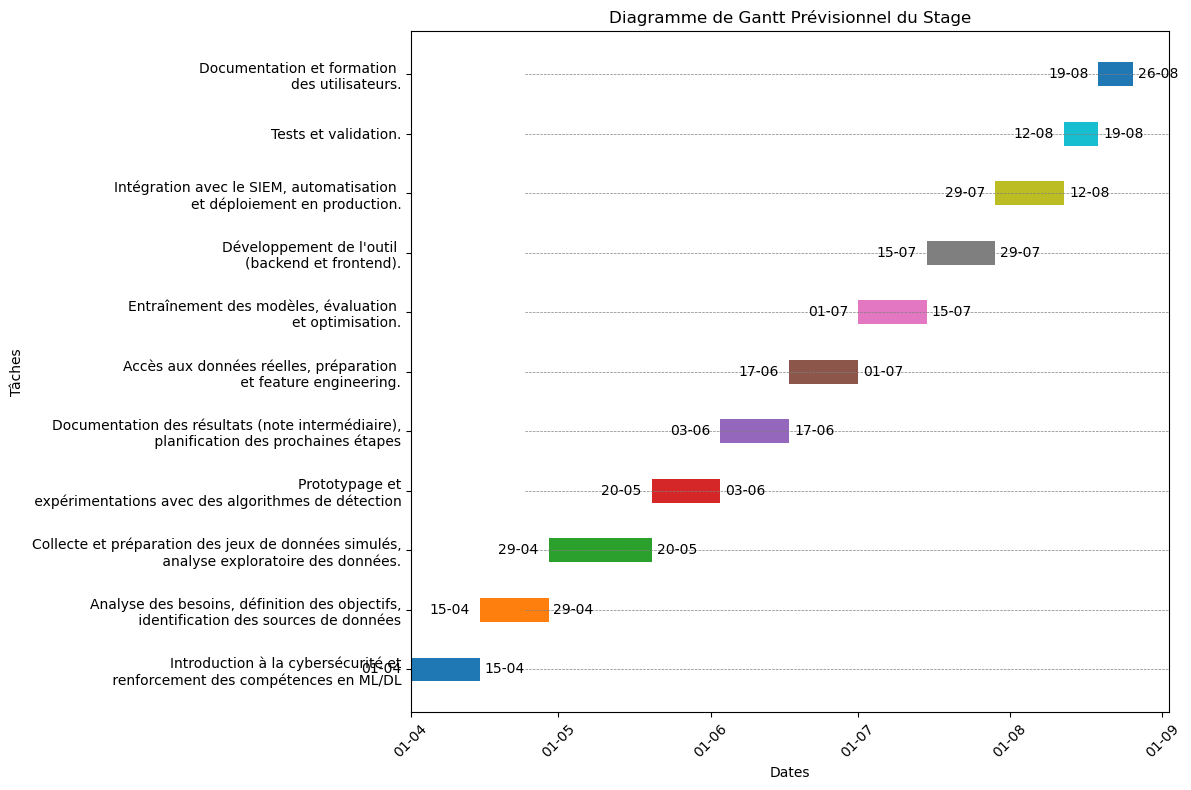
\includegraphics{figures/gantt.png}

}

\caption{Gant}

\end{figure}%

\subsubsection{Détails techniques des implémentations et
configurations}\label{duxe9tails-techniques-des-impluxe9mentations-et-configurations}

\subsubsection{Bibliographie et
références}\label{bibliographie-et-ruxe9fuxe9rences}

\phantomsection\label{refs}
\begin{CSLReferences}{1}{0}
\bibitem[\citeproctext]{ref-noauthor_57snssi03020ac_nodate}
{``{57SNSSI03020Ac} - {Analyste} Du {Security} {Operations} {Center}
({SOC}).''} n.d. \emph{Intranet INSEE}. Accessed August 7, 2024.
\url{https://intranet.insee.fr/jcms/32252877_DBFileDocument/fr/57snssi03020ac-analyste-du-security-operations-center-soc?details=true}.

\bibitem[\citeproctext]{ref-chio_machine_nodate}
Chio, Clarence, and David Freeman. n.d. {``Machine {Learning} Et
Sécurité {[}{Book}{]}.''} Accessed August 6, 2024.
\url{https://www.oreilly.com/library/view/machine-learning-et/9782412043561/}.

\bibitem[\citeproctext]{ref-noauthor_cybersecurite_2024}
{``Cybersécurité.''} 2024. \emph{Wikipédia}.
\url{https://fr.wikipedia.org/w/index.php?title=Cybers\%C3\%A9curit\%C3\%A9&oldid=215272230}.

\bibitem[\citeproctext]{ref-noauthor_dechiffrer_nodate}
{``Déchiffrer Le {Mag} 12 (Décembre 2023) - Version Pdf Accessible.''}
n.d. \emph{Intranet INSEE}. Accessed August 6, 2024.
\url{https://intranet.insee.fr/jcms/29406323_DBFileDocument/fr/dechiffrer-le-mag-12-decembre-2023-version-pdf-accessible?details=true}.

\bibitem[\citeproctext]{ref-noauthor_mi-2020-2_nodate}
{``{MI}-2020-2 {Carrieres} Informatiques {Insee} {CRCD}.''} n.d.
\emph{Intranet INSEE}. Accessed August 6, 2024.
\url{https://intranet.insee.fr/jcms/58667_DBFileDocument/fr/mi-2020-2-carrieres-informatiques-insee-crcd?details=true}.

\bibitem[\citeproctext]{ref-noauthor_mi-2020-2_nodate-1}
{``{MI}-2020-2 {Carrieres} Informatiques {Insee} {Rapport}.''} n.d.
\emph{Intranet INSEE}. Accessed August 6, 2024.
\url{https://intranet.insee.fr/jcms/58657_DBFileDocument/fr/mi-2020-2-carrieres-informatiques-insee-rapport?details=true}.

\bibitem[\citeproctext]{ref-noauthor_quest-ce_nodate}
{``Qu'est-Ce Que La Cybersécurité ?''} n.d. \emph{Cisco}. Accessed
August 6, 2024.
\url{https://www.cisco.com/c/fr_fr/products/security/what-is-cybersecurity.html}.

\bibitem[\citeproctext]{ref-noauthor_recommandations_nodate}
{``Recommandations Relatives à l'administration Sécurisée Des {SI}
{\textbar} {ANSSI}.''} n.d. Accessed August 7, 2024.
\url{https://cyber.gouv.fr/publications/recommandations-relatives-ladministration-securisee-des-si}.

\bibitem[\citeproctext]{ref-noauthor_reseau_2024}
{``Reseau · {Wiki} · {Domaine} Production Informatique / {DPII} Pour
{DSI} / {Documentation} Du {SI} · {GitLab}.''} 2024. \emph{GitLab}.
\url{https://gitlab.insee.fr/domaine-production-informatique/dpii-pour-dsi/documentation-du-si/-/wikis/Reseau}.

\end{CSLReferences}




\end{document}
